% Options for packages loaded elsewhere
\PassOptionsToPackage{unicode}{hyperref}
\PassOptionsToPackage{hyphens}{url}
%
\documentclass[
  12pt,
  oneside]{book}
\usepackage{lmodern}
\usepackage{setspace}
\usepackage{amsmath}
\usepackage{ifxetex,ifluatex}
\ifnum 0\ifxetex 1\fi\ifluatex 1\fi=0 % if pdftex
  \usepackage[T1]{fontenc}
  \usepackage[utf8]{inputenc}
  \usepackage{textcomp} % provide euro and other symbols
  \usepackage{amssymb}
\else % if luatex or xetex
  \usepackage{unicode-math}
  \defaultfontfeatures{Scale=MatchLowercase}
  \defaultfontfeatures[\rmfamily]{Ligatures=TeX,Scale=1}
\fi
% Use upquote if available, for straight quotes in verbatim environments
\IfFileExists{upquote.sty}{\usepackage{upquote}}{}
\IfFileExists{microtype.sty}{% use microtype if available
  \usepackage[]{microtype}
  \UseMicrotypeSet[protrusion]{basicmath} % disable protrusion for tt fonts
}{}
\makeatletter
\@ifundefined{KOMAClassName}{% if non-KOMA class
  \IfFileExists{parskip.sty}{%
    \usepackage{parskip}
  }{% else
    \setlength{\parindent}{0pt}
    \setlength{\parskip}{6pt plus 2pt minus 1pt}}
}{% if KOMA class
  \KOMAoptions{parskip=half}}
\makeatother
\usepackage{xcolor}
\IfFileExists{xurl.sty}{\usepackage{xurl}}{} % add URL line breaks if available
\IfFileExists{bookmark.sty}{\usepackage{bookmark}}{\usepackage{hyperref}}
\hypersetup{
  pdftitle={Spatial pattern mining of tech clusters of dynamics and industry mix based on quantitative methods in England area, UK},
  hidelinks,
  pdfcreator={LaTeX via pandoc}}
\urlstyle{same} % disable monospaced font for URLs
\usepackage[left=4cm, right=3cm, top=2.5cm, bottom=2.5cm]{geometry}
\usepackage{longtable,booktabs}
% Correct order of tables after \paragraph or \subparagraph
\usepackage{etoolbox}
\makeatletter
\patchcmd\longtable{\par}{\if@noskipsec\mbox{}\fi\par}{}{}
\makeatother
% Allow footnotes in longtable head/foot
\IfFileExists{footnotehyper.sty}{\usepackage{footnotehyper}}{\usepackage{footnote}}
\makesavenoteenv{longtable}
\usepackage{graphicx}
\makeatletter
\def\maxwidth{\ifdim\Gin@nat@width>\linewidth\linewidth\else\Gin@nat@width\fi}
\def\maxheight{\ifdim\Gin@nat@height>\textheight\textheight\else\Gin@nat@height\fi}
\makeatother
% Scale images if necessary, so that they will not overflow the page
% margins by default, and it is still possible to overwrite the defaults
% using explicit options in \includegraphics[width, height, ...]{}
\setkeys{Gin}{width=\maxwidth,height=\maxheight,keepaspectratio}
% Set default figure placement to htbp
\makeatletter
\def\fps@figure{htbp}
\makeatother
\setlength{\emergencystretch}{3em} % prevent overfull lines
\providecommand{\tightlist}{%
  \setlength{\itemsep}{0pt}\setlength{\parskip}{0pt}}
\setcounter{secnumdepth}{5}
\usepackage[none]{hyphenat}
\pagestyle{plain}
\raggedbottom
\usepackage[nottoc,notlot,notlof]{tocbibind}
\usepackage{pdfpages}
\usepackage[width=\textwidth]{caption}

\usepackage{fancyhdr}
\pagestyle{fancy}
\fancyhf{}
\setlength{\headheight}{15pt}%
\fancyhead[RO,RE]{\nouppercase{\leftmark}}
\fancyfoot[CO, CE] {\thepage}
\renewcommand{\headrulewidth}{0pt}
\renewcommand{\footrulewidth}{0pt}
\usepackage{booktabs}
\usepackage{longtable}
\usepackage{array}
\usepackage{multirow}
\usepackage{wrapfig}
\usepackage{float}
\usepackage{colortbl}
\usepackage{pdflscape}
\usepackage{tabu}
\usepackage{threeparttable}
\usepackage{threeparttablex}
\usepackage[normalem]{ulem}
\usepackage{makecell}
\usepackage{xcolor}
\ifluatex
  \usepackage{selnolig}  % disable illegal ligatures
\fi
\usepackage[style=apa,]{biblatex}
\addbibresource{book.bib}
\addbibresource{packages.bib}
\addbibresource{test.bib}

\title{Spatial pattern mining of tech clusters of dynamics and industry mix based on quantitative methods in England area, UK}
\author{Zeqiang Fang\\
~\\
CASA0012, MSc Spatial Data Science and Visualisation Dissertation\\
~\\
Supervisor: Dr Max Nathan\\
~\\
Repository: \url{https://fang-zeqiang.github.io/CASA0012-Dissertation/}\\
~\\
This dissertation is submitted in part requirement for the\\
MSc (Or MRes) in the Centre for Advanced Spatial Analysis,\\
Bartlett Faculty of the Built Environment, UCL\\
~\\
Word count: 8,000}
\date{2021-08-08}

\begin{document}
\maketitle

\setstretch{1.5}
\pagenumbering{roman}

\hypertarget{abstract}{%
\chapter*{Abstract}\label{abstract}}

Some abstract text

\pagenumbering{roman}

\hypertarget{declaration}{%
\chapter*{Declaration}\label{declaration}}

I, Zeqiang Fang, hereby declare that this dissertation is all my own original work and that all sources have been acknowledged. It is xxx words in length

\hypertarget{acknowledgements}{%
\chapter*{Acknowledgements}\label{acknowledgements}}

I would like to thank blah blah

% Trigger ToC creation in LaTeX
\setcounter{tocdepth}{3}
\tableofcontents
\listoffigures
\listoftables

\hypertarget{abbreviations}{%
\chapter*{Abbreviations}\label{abbreviations}}

\begin{table}
\centering
\begin{tabular}{ll}
\toprule
\textbf{Term} & \textbf{Abbreviation}\\
\midrule
Digital Elevation Model & DEM\\
Digital Surface Model & DSM\\
Digital Terrain Model & DTM\\
\bottomrule
\end{tabular}
\end{table}

\hypertarget{introduction}{%
\chapter{Introduction}\label{introduction}}

\pagenumbering{arabic} 

\hypertarget{background}{%
\section{Background}\label{background}}

\begin{enumerate}
\def\labelenumi{\arabic{enumi}.}
\tightlist
\item
  tech cluster development
\item
  dynamics cause better performance
\item
  industry clustering pattern and economics performances
\end{enumerate}

\hypertarget{research-question-and-objectives}{%
\section{Research Question and Objectives}\label{research-question-and-objectives}}

How does tech clusters' dynamics pattern change in UK from 1998 to 2018? / What factors can affect tech clusters' dynamics pattern change in UK?

To what extent will dynamic change affect tech clusters'performance?

\hypertarget{report-structure}{%
\section{Report Structure}\label{report-structure}}

\begin{enumerate}
\def\labelenumi{\arabic{enumi}.}
\tightlist
\item
  data clean
\item
  tech cluster recognition
\item
  dynamics index generation
\item
  hypothesis (OLS estimation)
\item
  regression
\item
  residual analysis
\item
  result interpretation
\end{enumerate}

\hypertarget{crossref}{%
\chapter{Literature Review}\label{crossref}}

\hypertarget{industry-cluster-tech-cluster}{%
\section{Industry Cluster \& Tech Cluster}\label{industry-cluster-tech-cluster}}

Tech clusters like Silicon Valley play a central role for modern innovation, business competitiveness, and economic performance. This paper reviews what constitutes a tech cluster, how they function internally, and the degree to which policy makers can purposefully foster them. We describe the growing influence of advanced technologies for businesses outside of traditional tech fields, the strains and backlash that tech clusters are experiencing, and emerging research questions for theory and empirical work.

\hypertarget{cluster-dynamics}{%
\section{Cluster Dynamics}\label{cluster-dynamics}}

Industrial dynamics and clusters: a survey, regional research. This article reviews clusters and their impact on the entry, exit, and growth of firms, as well as the literature supporting the evolutionary dynamics of cluster formation. This extensive review shows strong evidence that clusters promote the entry of manufacturers, but the evidence that clusters can promote the growth and survival of firms is rather weak. From a number of open-ended questions, this research extracts various future research paths that emphasize the importance of manufacturer heterogeneity and the exact mechanism that supports the localized economy.

\hypertarget{location-quotient}{%
\section{Location Quotient}\label{location-quotient}}

On average, companies in large cities are more productive. There are two main explanations: corporate choice (big cities strengthen competition and only allow the most productive people to survive) and agglomeration economies (big cities promote interaction and increase productivity), which may be strengthened by the natural advantages of localization. In order to distinguish them, we nested a general version of the easy-to-handle company selection model and a standard agglomeration model. Stronger choices in large cities cut the distribution of productivity to the left, while stronger gatherings move to the right and expand the distribution. Using this forecast, French firm-level data, and new quantile methods, we show that firm choices cannot explain differences in spatial productivity. The results are applicable to various departments, city size thresholds, institutional samples and regional definitions.

\hypertarget{how-location-affect-entry-pattern-in-ukglobal}{%
\section{How location affect entry pattern in UK/Global}\label{how-location-affect-entry-pattern-in-ukglobal}}

\hypertarget{how-time-affect-entry-pattern-in-ukglobal}{%
\section{How time affect entry pattern in UK/Global}\label{how-time-affect-entry-pattern-in-ukglobal}}

\hypertarget{other-factor-can-affect-dynamics-pattern-in-uk}{%
\section{Other factor can affect dynamics pattern in UK}\label{other-factor-can-affect-dynamics-pattern-in-uk}}

\hypertarget{methodology}{%
\chapter{Methodology}\label{methodology}}

\hypertarget{research-framework}{%
\section{Research Framework}\label{research-framework}}

\begin{enumerate}
\def\labelenumi{\arabic{enumi}.}
\tightlist
\item
  Data Clean \& Select
\item
  Identifying Tech Cluster
\item
  Measuring the Dynamics \& Industry Mix
\item
  Quantitative Method Research
\item
  Temporal Qualitative Analysis
\end{enumerate}

In this study, a data set containing all companies in UK will be cleaned and attribute selected, and technology companies will be identified and screened according to the classification and definition of technology companies on the official website of the British government. Before the quantitative study, this study is based on time and The spatial dimension counts the number of technology companies, and calculates the dynamic indicators of enterprise clusters and industrial combination indicators in a specific year and a specific region. Then this study conducts multiple regressions, univariate and bivariate variables Moran index testing to conduct spatial quantitative research, and finally combines Qualitative spatial pattern trend research on the spatial changes of indicators in three different time periods

在本研究中,包含所有英国公司的数据集会被进行数据清洗和属性选择,并且根据英国政府官网对于科技企业的分类定义来进行科技公司的识别与筛选;在定量研究前,本研究基于时间与空间维度对科技公司数量进行统计,并且计算出特定年份特定地区的企业集群动态指标与产业组合指标;紧接着本研究进行多元回归,单双变量的莫兰指数检测来进行空间定量研究,最后结合三个不同时间段的指标空间变化进行定性的空间模式趋势研究

\hypertarget{data-source-and-processing}{%
\section{Data Source and Processing}\label{data-source-and-processing}}

This raw dataset is collected from the core company data from Open Corporates master company database (Open Corporates, 2018). And the size of dataset accounts for 15 GB which is handled with \texttt{read\_stata} and \texttt{get\_chunk} function to read large data file in chunks, then increasing the reading speed. The ``primary uk sic 2007'' identification field is the basis of industry finding and the ``birth year'' is the key to measure dynamics variables . All rows whose these two values are empty are removed(17\% incorperate date is missing and sic code is complete).

\hypertarget{identifying-tech-cluster}{%
\section{Identifying Tech Cluster}\label{identifying-tech-cluster}}

For the identification of science and technology companies, this study introduces the main 2007 sic code table to judge the science and technology industry, referring to the classification method of the Science and Technology Classification data set on the ons.gov.uk website; in order to better identify science and technology companies for the UK The economic contribution is officially based on the 2007 British Standard Economic Activity Classification, combined with different data sources, to classify and label science and technology companies (Office for National Statistics, 2015).

\begin{table}

\caption{\label{tab:table-1}2007 sic code for science and technology industry (part)}
\centering
\begin{tabular}[t]{lrlll}
\toprule
SIC07 type & 5-digit SIC07 code & ...3 & Science and Technology category & Science and Technology topic\\
\midrule
Class & 26110 & ... & Digital Technologies & Computer \& Electronic manufacturing\\
Class & 58210 & ... & Digital Technologies & Digital \& Computer Services\\
Class & 62090 & ... & Digital Technologies & Digital \& Computer Services\\
Class & 63110 & ... & Digital Technologies & Digital \& Computer Services\\
Class & 27510 & ... & Other scientific/technological manufacture & Electrical Machinery manufacturing\\
\addlinespace
Class & 86230 & ... & Life Sciences \& Healthcare & Healthcare services\\
\bottomrule
\end{tabular}
\end{table}

This research refers to the science and technology classification table provided by the government. The technology indicator is used to position the technology industry of all industries, and a total of 168 sic codes for the technology industry in 2007 were obtained, accounting for about 16\% of all industry categories in the UK, including 5 industry categories such as Digital Technologies, Life Sciences \& Healthcare, Publishing \& Broadcasting , Other scientific/technological manufacture and Other scientific/technological services, details of the classification form will be attached in the attachment. There are almost 20\% firms in the raw data belonging to tech firms according to the method of category as mentioned above.

\hypertarget{quatitative-analysis-and-methods}{%
\section{Quatitative Analysis and Methods}\label{quatitative-analysis-and-methods}}

\hypertarget{time-range-selection}{%
\subsection{Time Range Selection}\label{time-range-selection}}

The reason why this research choose tech firms which incorporate from 1998 to 2018 is because
这20年来科技公司在英国的成立数量相比1998年以前明显走高正如图1所示

\begin{figure}
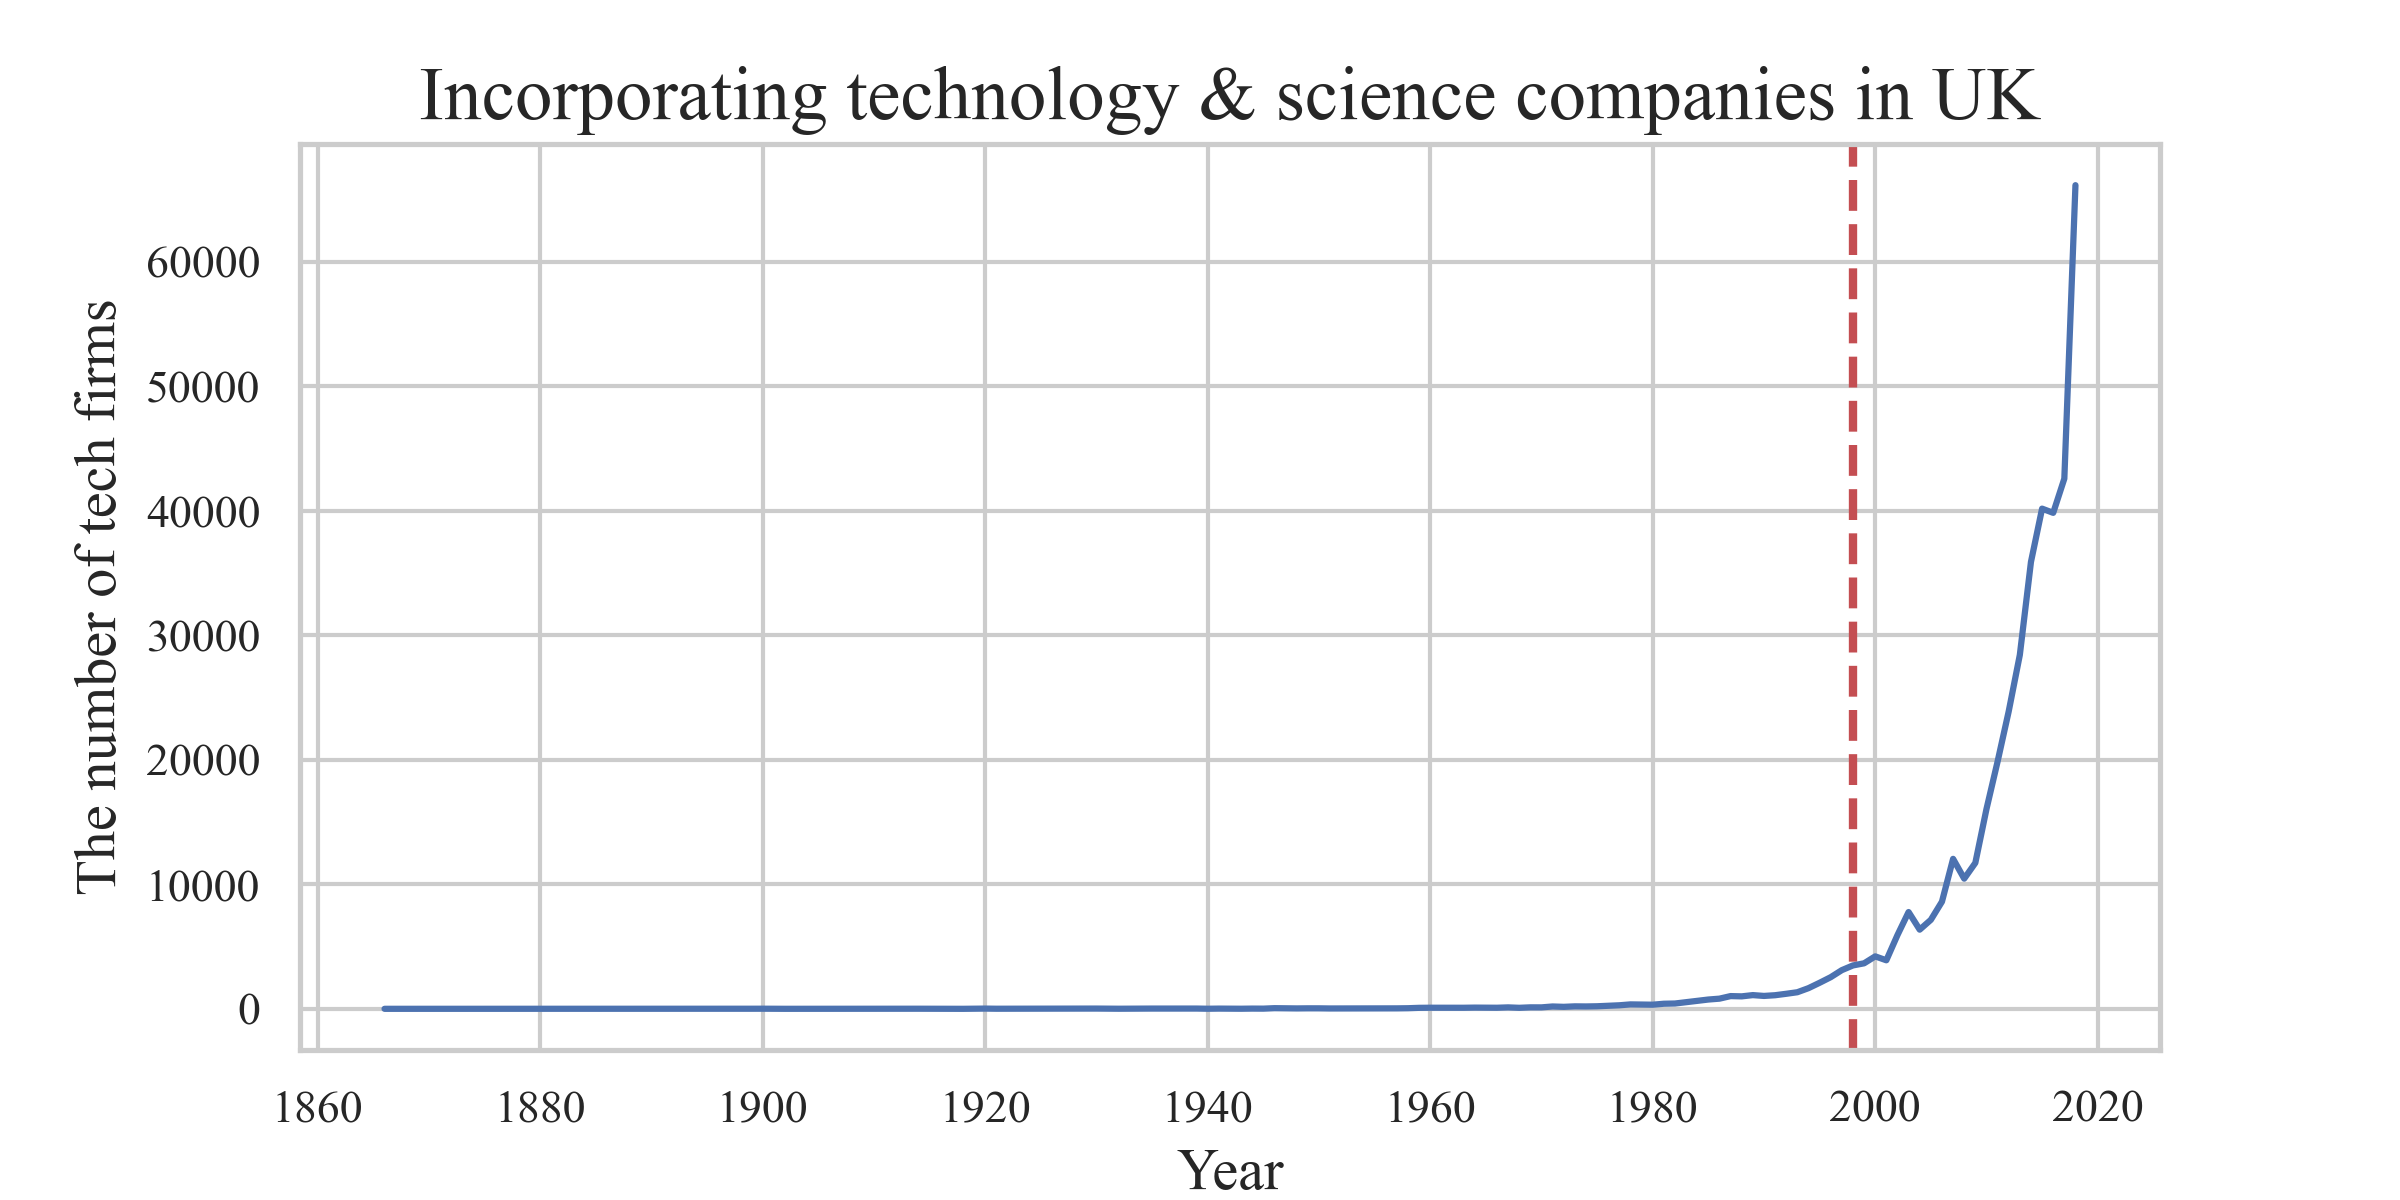
\includegraphics[width=1\linewidth]{/Users/fangzeqiang/Github/CASA0012-Dissertation/bookdown/general_images/figure1} \caption{Incorporating technology & science companies in UK}\label{fig:fig-1}
\end{figure}

\hypertarget{tech-cluster-identifying}{%
\subsection{Tech Cluster Identifying}\label{tech-cluster-identifying}}

What is ttwa?

The 228 areas forming the 2011 TTWAs, covering the whole of the UK, were defined in 2015 using 2011 Census commuting flow data, indicating home and workplace address. The TTWAs are based on aggregations of Lower Layer Super Output Areas (LSOA) in England and Wales, Data Zones (DZ) in Scotland, and Super Output Areas (SOA) in Northern Ireland and in some cases span country borders. There are six cross-border TTWAs, 149 in England, 18 in Wales, 45 in Scotland and 10 in Northern Ireland (\ldots,\ldots).

\begin{itemize}
\tightlist
\item
  Why choose TTWA?
\end{itemize}

This geographical division can better reflect the relationship between population, company and work (\ldots,\ldots)

\begin{itemize}
\tightlist
\item
  Why ttwa can work as a firms' cluster?
\end{itemize}

Some researchers have found\ldots{} (\ldots,\ldots)

\hypertarget{dynamics-measuring-index}{%
\subsection{Dynamics Measuring Index}\label{dynamics-measuring-index}}

衡量一个集群的动态变化程度需要计算出科技集群的进入率,计算方法如下
这里参考了其他研究者的计算方法(\ldots,\ldots)

\[ Entry\ Rate_{i,t} = \frac{Incorporating\ Firms_{i,t}}{Total\  Firms_{i}} \]
Where \(i\) means location(travel to work area), \(t\) means year

\hypertarget{industry-mix-measuring-index}{%
\subsection{Industry Mix Measuring Index}\label{industry-mix-measuring-index}}

衡量一个集群地区的产业集中程度需要计算出科技集群的Herfindahl-Hirschman Index或者location quotient,这里只采用前者的方法是因为缺失相应地区年份对应的受雇人员数据,故采用前者进行指标计算,这里参考了其他研究者的计算方法(\ldots,\ldots),计算方法如下

\[ Herfindahl-Hirschman \ Index_{\ i,t} = \sum_1^k (\frac{Tech\ Firms_{i,t,k}}{Total\ Tech\ Firms_{i,t}})^2 \]
Where \(k\) represents the \(k\)th industry in location \(i\) and year \(t\). \(Tech Firms\) means the number of tech companies and \(Total Tech Firms\) represents the number of total tech firms in a specific location and year.

赫芬达尔---赫希曼指数 {[}1{]} (Herfindahl-Hirschman Index,简称HHI),简称赫芬达尔指数,是一种测量产业集中度的综合指数。它是指一个行业中各市场竞争主体所占行业总收入或总资产百分比的平方和,用来计量市场份额的变化,即市场中厂商规模的离散度。

赫芬达尔一赫希曼指数是计算某一市场上50家最大企业(如果少于50家企业就是所有企业)每家企业市场占有份额(取百分之的分子)的平方之和。显然, HHI越大,表示市场集中程度越高,垄断程度越高。该指数不仅能反映市场内大企业的市场份额,而且能反映大企业之外的市场结构,因此,能更准确地反映大企业对市场的影响程度。

\hypertarget{dynamics-and-performance-analysis}{%
\subsection{Dynamics and Performance Analysis}\label{dynamics-and-performance-analysis}}

\hypertarget{limitations}{%
\section{Limitations}\label{limitations}}

\begin{enumerate}
\def\labelenumi{\arabic{enumi}.}
\item
  missing data
  \texttt{diss\_year} have 99\% missing value
\item
  ttwa
\end{enumerate}

\begin{itemize}
\tightlist
\item
  ttwa might not be a data-driven method
\item
  ttwa的时间局限性,因为是2015年统计的
\item
  ttwa的变化(Ozkul,2014)
\end{itemize}

Ozkul, B., 2014. Changing home-to-work travel in England and Wales. Regional Studies, Regional Science, 1(1), pp.32-39.

\hypertarget{herfindahl-hirschman-index}{%
\section{1. Herfindahl-Hirschman Index}\label{herfindahl-hirschman-index}}

\hypertarget{ethical-statement}{%
\section{Ethical Statement}\label{ethical-statement}}

The data for this project comes from OpenCorporates, a firm which aggregates company-level data from around the world {[}link to their website{]}. In this case, OpenCorporates have taken data from the UK Companies House register {[}link to Companies House{]}. As detailed by Nathan and Rosso (2015), all limited companies in the UK need to registers with Companies House when they are set up, and provide annual returns and financial statements. These include details of directors and company secretary, registered office address, shares and shareholders, as well as company type and principal business activity. Thus, all the data used here is already in the public domain.

The research objectives are tech firms in the UK for this project and the individual data will not be collected and measured in this project. For issues of deanonymisation or privacy, traceable information such as the real companies name and ID will not be utilised in the research. The raw data will be cleaned and filtered by several key variables include industries instead of the company's name or other sensitive information before doing the research. Through data cleaning, pre-processing, desensitisation or other processing methods, the risks of damage to company interests (such as social reputation, economic benefits and etc.) will be mitigated to an as low as possible level in the research process.

Besides, this project will not cause discrimination of industries or job categories. The final analysis results, such as the different industry concentration in each region, will not deepen some people's stereotypes and prejudices about the region (This content will be fully discussed in the project discussion section). It is necessary to point out and declare the objectivity of the analysis and the non-absoluteness of the results in the disclaimer. Consider the feelings of people and governments in different parts of the UK, this research will prevent the influence of personal preferences and subjective emotions.

The leakage of companies' name and information will be protected. For example, in the reflection of the results section of academic research, the name and related information of the companies that moved may be revealed. Although this information may be open to the public you need to know that this information may be used by people with other ulterior motives. This project will desensitise the company name and information at the stage of chart presentation, such as using A, B, and C to replace them to achieve this purpose.

\hypertarget{results}{%
\chapter{Results}\label{results}}

\hypertarget{visualisation-and-analysis-of-tech-cluster}{%
\section{Visualisation and Analysis of Tech Cluster}\label{visualisation-and-analysis-of-tech-cluster}}

\hypertarget{distribution}{%
\subsection{Distribution}\label{distribution}}

\hypertarget{descriptive-analysis}{%
\subsection{Descriptive Analysis}\label{descriptive-analysis}}

\hypertarget{visualisation-and-analysis-of-dynamics}{%
\section{Visualisation and Analysis of Dynamics}\label{visualisation-and-analysis-of-dynamics}}

\hypertarget{regression}{%
\subsection{Regression}\label{regression}}

\hypertarget{discussion}{%
\chapter{Discussion}\label{discussion}}

Short introduction to the chapter, reviewing the previous chapter and detailing what this one aims to achieve and build upon.

To be done

\hypertarget{research-significance}{%
\section{Research significance}\label{research-significance}}

\hypertarget{global-development-goals}{%
\subsection{Global development goals}\label{global-development-goals}}

\hypertarget{local-policy}{%
\subsection{Local policy}\label{local-policy}}

\hypertarget{academic-research}{%
\subsection{Academic research}\label{academic-research}}

\hypertarget{limitations-1}{%
\section{Limitations}\label{limitations-1}}

To be done

\hypertarget{transferability}{%
\section{Transferability}\label{transferability}}

To be done

\hypertarget{conclusion}{%
\chapter{Conclusion}\label{conclusion}}

Short introduction to the chapter, reviewing the previous chapter and detailing what this one aims to achieve and build upon.

To be done

\hypertarget{references}{%
\chapter*{References}\label{references}}
\addcontentsline{toc}{chapter}{References}

a b c d e f g h i j k l m n o p q r s t u v w x y z

Combes, P.-P., Duranton, G., Gobillon, L., Puga, D. and Roux, S. (2012),The Productivity Advantages of Large Cities: Distinguishing AgglomerationFrom Firm Selection. Econometrica, 80: 2543-2594.https://doi.org/10.3982/ECTA84427

Frenken, K., Cefis, E., \& Stam, E. (2015). Industrial Dynamicsand Clusters: A Survey. Regional Studies, 49(1), 10-27.doi:10.1080/00343404.2014.904505

Kerr, William R., and Frederic Robert-Nicoud. 2020. ``Tech Clusters.''Journal of Economic Perspectives, 34 (3): 50-76.https://www.aeaweb.org/articles?id=10.1257/jep.34.3.50

Open Corporates. (2018), The core company data from OpenCorporates master company database, electronic dataset, OpenCorporates Data Dictionary, viewed 12 June 2021, \url{https://opencorporates.com/}.

Office for National Statistics, 2015. Identifying Science and Technology Businesses in Official Statistics. {[}online{]} London, UK: Office for National Statistics, pp.10-14. Available at: \url{https://webarchive.nationalarchives.gov.uk/20160105170025/http://www.ons.gov.uk/ons/site-information/using-the-website/rss-news-feeds/index.html} {[}Accessed 28 July 2021{]}.

\addcontentsline{toc}{chapter}{Bibliography}
\printbibliography

\hypertarget{appendix-a-classification-form}{%
\chapter*{Appendix A Classification Form}\label{appendix-a-classification-form}}
\addcontentsline{toc}{chapter}{Appendix A Classification Form}

\addtocontents{toc}{\protect\setcounter{tocdepth}{0}}

\hypertarget{science-and-technology-classification}{%
\section*{Science and Technology Classification}\label{science-and-technology-classification}}

\hypertarget{appendix-b-proposal}{%
\chapter*{Appendix B Proposal}\label{appendix-b-proposal}}

\addtocontents{toc}{\protect\setcounter{tocdepth}{3}}
\enddocument

\printbibliography

\end{document}
